\documentclass[tikz,border=3pt]{standalone}
\usepackage[utf8]{inputenc}
\usepackage[T1]{fontenc}
\usepackage{lmodern}
\renewcommand{\familydefault}{\sfdefault}
\usepackage{sansmath}\sansmath
\usepackage{chemfig}
\usepackage{pgfplots}\pgfplotsset{compat=1.18,/pgf/number format/use comma,/pgf/number format/1000 sep={.}}
\usetikzlibrary{arrows.meta,calc,positioning,decorations.pathmorphing,patterns}
% paleta del sitio
\definecolor{nar}{HTML}{E8680C}\definecolor{narc}{HTML}{FFB35C}\definecolor{hielo}{HTML}{FFF3E8}
\definecolor{tinta}{HTML}{1D1D1F}\definecolor{gris}{HTML}{6E6E73}\definecolor{lila}{HTML}{7C5CF0}
\definecolor{azul}{HTML}{2F6FD6}\definecolor{menta}{HTML}{17A673}\definecolor{coral}{HTML}{E8342A}
\begin{document}
\newcommand{\jirafa}[5]{% x, y (cuerpo), largo del cuello, relleno, borde
\begin{scope}[shift={(#1,#2)}]
\foreach \lx in {-0.22,-0.1,0.1,0.22} \draw[#5,line width=1.6pt] (\lx,-0.05) -- (\lx,-0.5);
\draw[#5,line width=4.2pt,line cap=round] (0.2,0.06) -- ++(72:#3);
\draw[#4,line width=2.6pt,line cap=round] (0.2,0.06) -- ++(72:#3);
\fill[#4,draw=#5,thick] (0,0) ellipse (0.33 and 0.17);
\fill[#4,draw=#5,thick] ($(0.2,0.06)+(72:#3)+(0.09,0)$) ellipse (0.15 and 0.075);
\end{scope}}
\newcommand{\arbol}[3]{% x, y base, alto
\fill[nar!60!black] (#1-0.06,#2) rectangle (#1+0.06,#2+#3);
\fill[menta!75] (#1,#2+#3+0.25) ellipse (0.5 and 0.33);}
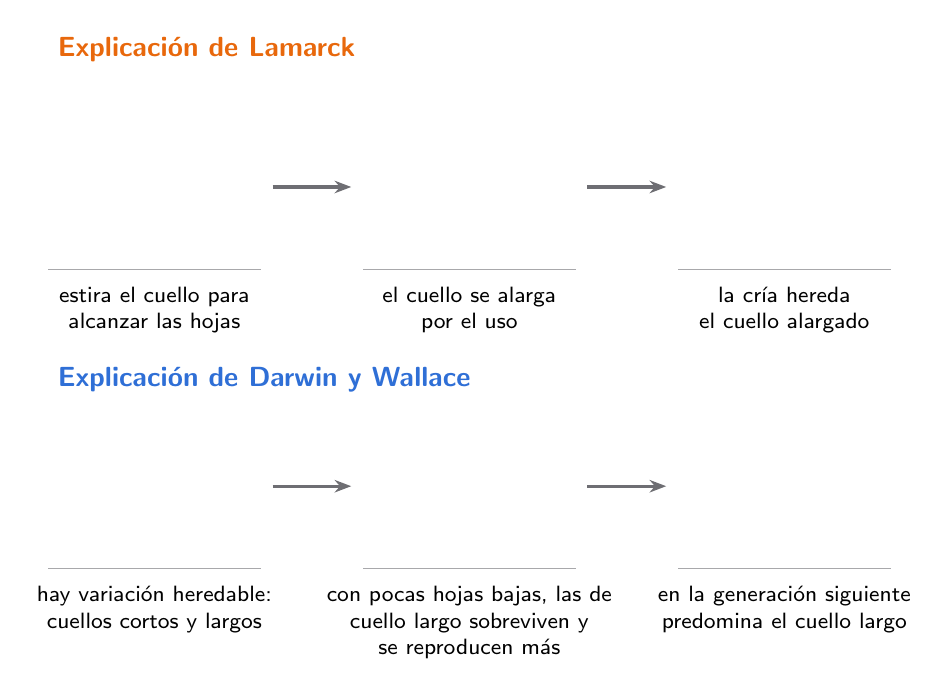
\begin{tikzpicture}[font=\small]
\tikzset{flecha/.style={-{Stealth[length=6pt]},gris,very thick}}
% ---------- Lamarck ----------
\node[anchor=west,font=\bfseries,text=nar] at (-1.1,5.75) {Explicación de Lamarck};
\foreach \c in {0,4,8} \draw[gris!60] (\c-1.1,2.95) -- (\c+1.6,2.95);
\jirafa{0}{3.45}{0.75}{narc}{nar}\arbol{1.1}{2.95}{1.6}
\jirafa{4}{3.45}{1.3}{narc}{nar}\arbol{5.1}{2.95}{1.6}
\jirafa{8}{3.45}{1.3}{narc}{nar}
\begin{scope}[shift={(8.95,3.2)},scale=0.62]\jirafa{0}{0}{1.15}{narc}{nar}\end{scope}
\draw[flecha] (1.75,4.0) -- (2.75,4.0);
\draw[flecha] (5.75,4.0) -- (6.75,4.0);
\node[align=center,font=\footnotesize,anchor=north] at (0.25,2.85) {estira el cuello para\\alcanzar las hojas};
\node[align=center,font=\footnotesize,anchor=north] at (4.25,2.85) {el cuello se alarga\\por el uso};
\node[align=center,font=\footnotesize,anchor=north] at (8.25,2.85) {la cría hereda\\el cuello alargado};
% ---------- Darwin ----------
\node[anchor=west,font=\bfseries,text=azul] at (-1.1,1.55) {Explicación de Darwin y Wallace};
\foreach \c in {0,4,8} \draw[gris!60] (\c-1.1,-0.85) -- (\c+1.6,-0.85);
\jirafa{-0.75}{-0.35}{0.55}{narc}{nar}\jirafa{0.05}{-0.35}{0.9}{narc}{nar}\jirafa{0.85}{-0.35}{1.3}{narc}{nar}
\jirafa{3.25}{-0.35}{0.55}{gris!25}{gris!70}\jirafa{4.05}{-0.35}{0.9}{gris!25}{gris!70}\jirafa{4.85}{-0.35}{1.3}{narc}{nar}
\jirafa{7.25}{-0.35}{1.3}{narc}{nar}\jirafa{8.05}{-0.35}{1.25}{narc}{nar}\jirafa{8.85}{-0.35}{0.9}{narc}{nar}
\draw[flecha] (1.75,0.2) -- (2.75,0.2);
\draw[flecha] (5.75,0.2) -- (6.75,0.2);
\node[align=center,font=\footnotesize,anchor=north] at (0.25,-0.95) {hay variación heredable:\\cuellos cortos y largos};
\node[align=center,font=\footnotesize,anchor=north] at (4.25,-0.95) {con pocas hojas bajas, las de\\cuello largo sobreviven y\\se reproducen más};
\node[align=center,font=\footnotesize,anchor=north] at (8.25,-0.95) {en la generación siguiente\\predomina el cuello largo};
\end{tikzpicture}
\end{document}
